\documentclass[11pt]{standalone}
\usepackage{pgf, tikz}
\usetikzlibrary{arrows, automata}
\begin{document}
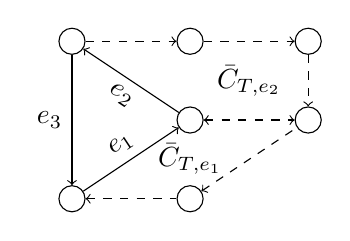
\begin{tikzpicture} [align=center]
\path (0,0) node[circle, draw] (v0) {}
	  (1.5,1) node[circle, draw] (v1) {}
	  (0,2) node[circle, draw] (v2) {}
	  (3,1) node[circle, draw] (v3) {}
	  (1.5,0) node[circle, draw] (v4) {}
	  (1.5,2) node[circle, draw] (v5) {}
	  (3,2) node[circle, draw] (v6) {}
	  
(1.5,0.5) node (c1) {$\bar{C}_{T,e_1}$}
(2.25,1.5) node (c2) {$\bar{C}_{T,e_2}$};

\draw[->] (v0) to node [sloped, anchor=center, above] {$e_1$} (v1);
\draw[->] (v1) to node [sloped, anchor=center, below] {$e_2$} (v2);
\draw[->] (v2) to node [left] {$e_3$} (v0);

\draw[dashed, <-] (v0) to (v4);
\draw[dashed, <-] (v4) to (v3);
\draw[dashed, <->] (v1) to (v3);
\draw[dashed, ->] (v2) to (v5);
\draw[dashed, ->] (v5) to (v6);
\draw[dashed, ->] (v6) to (v3);
	  
\end{tikzpicture}
\end{document}